% \documentclass[aspectratio=169,notes]{beamer}
\documentclass[aspectratio=169]{beamer}
\usetheme[faculty=phil]{fibeamer}
\usepackage{polyglossia}
\setmainlanguage{english} %% main locale instead of `english`, you
%% can typeset the presentation in either Czech or Slovak,
%% respectively.
\setotherlanguages{russian} %% The additional keys allow
%%
%%   \begin{otherlanguage}{czech}   ... \end{otherlanguage}
%%   \begin{otherlanguage}{slovak}  ... \end{otherlanguage}
%%
%% These macros specify information about the presentation
\title[Introduction to Robotics (In2Ro)]{Introduction to Robotics, Homework 1} %% that will be typeset on the
\subtitle{The AR-601M arm
\\ Forward and inverse kinematics, Jacobian, singularities \\ \  } %% title page.
\author{Oleg Bulichev}
%% These additional packages are used within the document:
\usepackage{ragged2e}  % `\justifying` text
\usepackage{booktabs}  % Tables
\usepackage{tabularx}
\usepackage{tikz}      % Diagrams
\usetikzlibrary{calc, shapes, backgrounds, trees, positioning, arrows.meta}
\usetikzlibrary{decorations.pathreplacing,calligraphy,calc,graphs}
\usepackage{amsmath, amssymb}
\usepackage{url}       % `\url`s
\usepackage{listings}  % Code listings
\usepackage{floatrow}
\usepackage{subcaption}
\usepackage{mathtools}
\usepackage{todonotes}
\usepackage{fontspec}
\usepackage{multicol}
\usepackage{pdfpages}
\usepackage{wrapfig}
\usepackage{qrcode}
\usepackage{animate}
\usepackage{booktabs}
\usepackage{multirow}
\usepackage{graphicx}
\usepackage{colortbl}

\graphicspath{{resources/}}
\frenchspacing

\setbeamertemplate{caption}{\raggedright\insertcaption\par}
\usetikzlibrary{graphs}

% \usepackage[backend=biber,style=ieee,autocite=footnote]{biblatex}
% \addbibresource{biblio.bib}
% \DefineBibliographyStrings{english}{%
%   bibliography = {References},}

\newcommand{\oleg}[2][] {\todo[color=red, #1] {OLEG:\\ #2}}
\newcommand{\fbckg}[1]{\usebackgroundtemplate{\includegraphics[width=\paperwidth]{#1}}}%frame background

\usepackage[framemethod=TikZ]{mdframed}
\newcommand{\dbox}[1]{
\begin{mdframed}[roundcorner=3pt, backgroundcolor=yellow, linewidth=0]
\vspace{1mm}
{#1}
\vspace{1mm}
\end{mdframed}
}

\begin{document}
\setlength{\abovedisplayskip}{0pt}
\setlength{\belowdisplayskip}{0pt}
\setlength{\abovedisplayshortskip}{0pt}
\setlength{\belowdisplayshortskip}{0pt}

\fbckg{fibeamer/figs/title_page.png}
\frame[c]{\setcounter{framenumber}{0}
    \usebeamerfont{title}%
    \usebeamercolor[fg]{title}%
    \begin{minipage}[b][6.5\baselineskip][b]{\textwidth}%
        \textcolor{black}{\raggedright\inserttitle}
    \end{minipage}
    % \vskip-1.5\baselineskip

    \usebeamerfont{subtitle}%
    \usebeamercolor[fg]{framesubtitle}%
    \begin{minipage}[b][3\baselineskip][b]{\textwidth}
        \raggedright%
        \insertsubtitle%
    \end{minipage}
    \vskip.25\baselineskip
}

\fbckg{fibeamer/figs/common.png}

%% AR-601M arm -- kinematic scheme, drawn from the factor chain (Task 1):
%%   0T6 = Rz(t1) Tz(l1) Rz(10deg*b) Ry(t2) Ty(-l2*b) Rx(t3) Tz(-l3)
%%         Rz(t4) Ry(t5) Rx(t6) Tx(l4)
%% An original schematic, not a redraw of the source photograph. \input
%% this file from both the deck (F03) and the handout; it only defines
%% \arsixonescheme, it draws nothing on its own.
%%
%% Uses tikz libraries calc, positioning, arrows.meta -- all already
%% loaded by both documents' preambles.
\newcommand{\arsixonescheme}{%
\begin{tikzpicture}[>=Latex, line width=0.7pt, scale=0.8,
    axis/.style={<->, thick},
    offset/.style={->, thick, blue!55!black},
    frame/.style={->, thick, black!70}]
  \coordinate (O) at (0,0);
  \coordinate (A) at (0,4.2);
  \coordinate (B) at (2.6,4.2);
  \coordinate (C) at (2.6,1.6);
  \coordinate (T) at (4.6,0.4);

  % base frame, at the fixed shoulder base
  \draw[frame] (O) -- ++(0.5,0) node[right] {\scriptsize $x_0$};
  \draw[frame] (O) -- ++(0,0.5) node[above] {\scriptsize $z_0$};
  \node[below=2pt] at (O) {\scriptsize base};
  \draw[axis] ($(O)+(1.1,-0.4)$) -- ++(0,0.8) node[right] {\scriptsize $t_1\,(z)$};

  % l1: fixed offset up to the shoulder -- label to the left, clear of t1
  \draw[offset] (O) -- (A) node[midway, left=2pt] {\scriptsize $l_1$};

  % fixed 10 degree shoulder tilt about z (not a joint)
  \draw[thin] (A) ++(160:0.45) arc (160:70:0.45);
  \node[above, align=center] at ($(A)+(0,0.7)$)
    {\scriptsize $10^\circ$ tilt\\[-2pt]\scriptsize(fixed)};

  % t2 about y -- label above the arrow
  \draw[axis] ($(A)+(0.9,0)$) -- ++(0.7,0) node[above] {\scriptsize $t_2\,(y)$};
  % l2 along -y*b -- label below the A-B segment
  \draw[offset] (A) -- (B) node[midway, below=2pt] {\scriptsize $l_2\,(-y{\cdot}b)$};

  % t3 about x -- axis out of the page, drawn as a target glyph
  \draw (B) circle (2.2pt); \fill (B) circle (0.6pt);
  \node[above right] at (B) {\scriptsize $t_3\,(x)$};

  % l3: down to the wrist centre -- label to the right of the segment
  \draw[offset] (B) -- (C) node[midway, right=2pt] {\scriptsize $l_3$};

  % wrist centre: t4, t5, t6 share this one point (no offset between them)
  \fill (C) circle (1.6pt);
  \node[above left=1pt] at (C) {\scriptsize wrist centre};

  % t4 (z), t5 (y), t6 (x) fanned well clear of C, of each other, of l3
  % above and l4 below-right, and of the t1/base cluster near the origin
  \draw[axis] ($(C)+(-1.0,0.85)$) -- ++(0,0.7) node[left] {\scriptsize $t_4\,(z)$};
  \draw[axis] ($(C)+(-1.55,-0.1)$) -- ++(0.7,0) node[below] {\scriptsize $t_5\,(y)$};
  \draw ($(C)+(-0.25,-1.3)$) circle (2.2pt); \fill ($(C)+(-0.25,-1.3)$) circle (0.6pt);
  \node[below] at ($(C)+(-0.25,-1.3)$) {\scriptsize $t_6\,(x)$};

  % l4: offset to the tool frame
  \draw[offset, dashed] (C) -- (T) node[midway, below=3pt] {\scriptsize $l_4\,(x)$};
  \draw[frame] (T) -- ++(0.5,0.2) node[right] {\scriptsize $x_6$};
  \draw[frame] (T) -- ++(-0.1,0.5) node[above] {\scriptsize $z_6$};
  \node[below] at (T) {\scriptsize tool};

  % arm mirror, as a note rather than a second drawing
  \node[align=left, font=\scriptsize, text width=3.4cm] at (7.4,2.6)
    {$b=+1$ shown (right arm).\\ $b=-1$ mirrors $l_2$ and the shoulder
     tilt about $z$ (left arm).};
\end{tikzpicture}%
}


\begin{frame}[t]{What this homework is}
\framesubtitle{One arm, six tasks, eighteen hours}
    AR-601M is a 41-DOF humanoid robot. This homework treats one of its two arms in
    isolation: a 6-DOF serial chain, shoulder to tool, with a spherical wrist.
    \medskip

    \begin{itemize}
        \item \textbf{Forward} kinematics: joint angles $\to$ tool pose.
        \item \textbf{Inverse} kinematics, analytical and numerical: tool pose $\to$ joint
              angles.
        \item The \textbf{Jacobian}, and where it loses rank: \textbf{singularities}.
    \end{itemize}
    \medskip

    About 18 hours of work covering weeks 1--3. This deck is a pointer; the full statement,
    with every derivation, requirement and hint, is the handout linked on the last frame.
\end{frame}

\begin{frame}[t]{The mechanism: AR-601M}
    \begin{figure}[H]
        \begin{subfigure}[t]{0.49\textwidth}
            \centering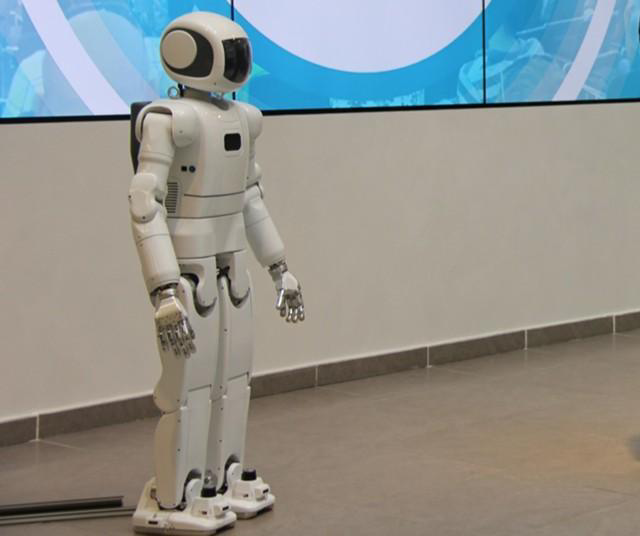
\includegraphics[height=4.2cm,width=1\textwidth,keepaspectratio]{ar601m_robot.png}
            \caption{The AR-601M arm.}
            \label{fig:ar601m_robot}
        \end{subfigure}
        \begin{subfigure}[t]{0.49\textwidth}
            \centering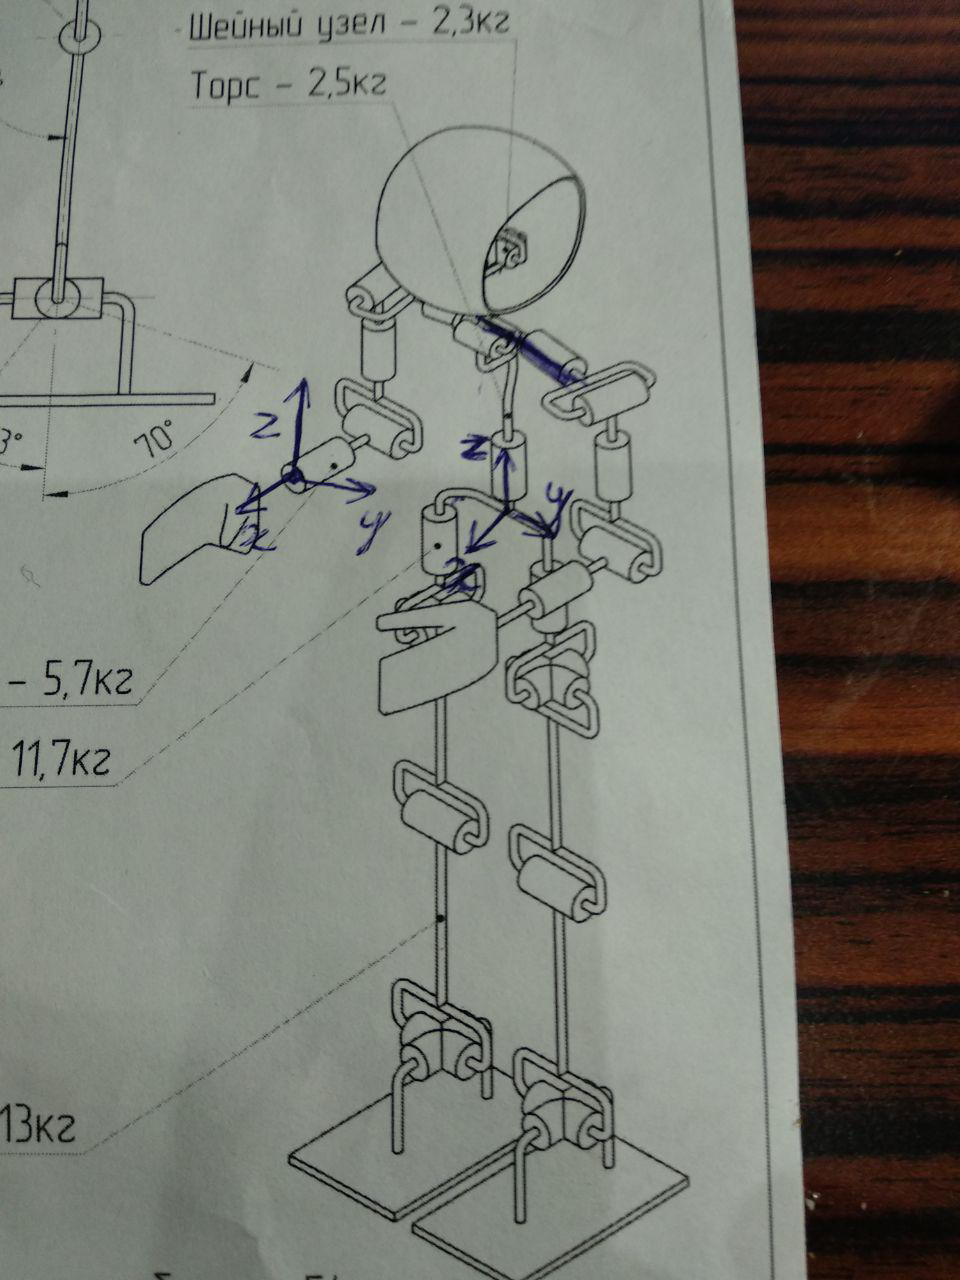
\includegraphics[height=4.2cm,width=1\textwidth,keepaspectratio]{ar601m_scheme.png}
            \caption{The blueprint, annotated in blue.}
            \label{fig:ar601m_scheme}
        \end{subfigure}

        \caption{The robot, and the blueprint it is modelled from; lengths are not
        legible on the blueprint, see handout \S2.}
        \label{fig:ar601m_pair}
    \end{figure}
\end{frame}

\begin{frame}[t]{The kinematic scheme and the chain}
\framesubtitle{${}^0T_6 = R_z(t_1)\,T_z(l_1)\,R_z(10^\circ b)\,R_y(t_2)\,T_y(-l_2 b)\,R_x(t_3)\,T_z(-l_3)\,R_z(t_4)\,R_y(t_5)\,R_x(t_6)\,T_x(l_4)$}
    \vspace{-0.6cm}
    \begin{figure}[H]
        \centering\arsixonescheme
        \label{fig:scheme_deck}
    \end{figure}
\end{frame}

\begin{frame}[t]{What you will be able to do}
    \begin{multicols}{2}
        \begin{itemize}
            \item Derive and implement forward kinematics for a serial chain with a
                  spherical wrist.
            \item Solve an inverse-kinematics target analytically, in closed form, keeping
                  every branch, not just the first one found.
            \item Solve the same target numerically and reconcile the answer against the
                  analytical branches.
            \item Build a manipulator Jacobian two independent ways and locate where it
                  loses rank.
        \end{itemize}
    \end{multicols}
\end{frame}

\begin{frame}[t]{The six tasks}
    \begin{multicols}{2}
        \begin{itemize}
            \item \textbf{1.} Kinematic model
            \item \textbf{2.} FK: angles $\to$ arm and pose
            \item \textbf{3.} IK: pose $\to$ every valid arm
            \item \textbf{4.} Numerical inverse kinematics
            \item \textbf{5.} Jacobian
            \item \textbf{6.} Singularity and branch-count maps
        \end{itemize}
    \end{multicols}
    \medskip

    Visualize Task 2's arm and transform, Task 3's unique valid branches, and
    Task 6's conditioning and fixed-orientation branch counts. Full requirements
    are in handout \S4.
\end{frame}

\begin{frame}[t]{What you hand in}
    \begin{block}{The packaging contract}
        \begin{itemize}
            \item A \texttt{pixi.toml} or a \texttt{Dockerfile} at the repository root.
            \item One command reproduces the report's numbers, example images and
                  maps from a clean checkout.
            \item Three functions, exactly these roles: \texttt{FK(q, robot)},
                  \texttt{IK(T, robot)}, \texttt{Jacobian(q, robot)} --- any language, the
                  same three signatures.
        \end{itemize}
    \end{block}
    \medskip

    Packaging is what is graded, not the language used to write it.
\end{frame}

\begin{frame}[t]{The full statement}
    \begin{columns}[T,onlytextwidth]
        \begin{column}{0.69\textwidth}
            Everything above is a pointer. The handout has every derivation, every
            requirement and every hint.
            \medskip

            Read handout \S3 and \S4 before writing any code.
            \medskip

            \href{https://github.com/Lupasic/In2Ro_MIPT_2026/blob/main/slides/homework/W01/resources/hw01_handout.pdf}{hw01\_handout.pdf on GitHub}
        \end{column}
        \begin{column}{0.29\textwidth}
            \begin{figure}[H]
                \centering
                \qrcode[height=3cm]{https://github.com/Lupasic/In2Ro_MIPT_2026/blob/main/slides/homework/W01/resources/hw01_handout.pdf}
                \caption*{\textbf{The handout}}
                \label{fig:qrcode_handout}
            \end{figure}
        \end{column}
    \end{columns}
\end{frame}

\fbckg{fibeamer/figs/last_page.png}
\frame[plain]{}

\end{document}
